\documentclass[tikz]{standalone}
\usetikzlibrary{positioning}

\begin{document}
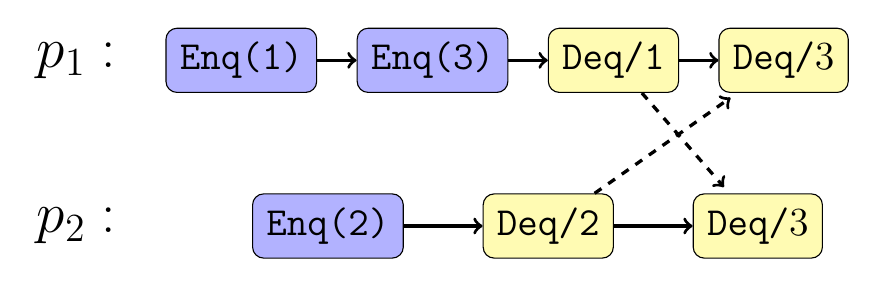
\begin{tikzpicture}
\tikzset{
  enq-op/.style = {rectangle, rounded corners, fill = blue!30, draw, font = \Large, inner sep = 5pt},
  deq-op/.style = {rectangle, rounded corners, fill = yellow!30, draw, font = \Large, inner sep = 5pt},
  process/.style = {font = \huge},
  po/.style = {->, very thick},
  vis/.style = {->, shorten >= 3pt, very thick, dashed}
}

  \node (p1) [process] {$p_1:$};
  \node (p1-enq1) [enq-op, right = 0.5cm of p1] {\texttt{Enq(1)}};
  \node (p1-enq3) [enq-op, right = 0.5cm of p1-enq1] {\texttt{Enq(3)}};
  \node (p1-deq1) [deq-op, right = 0.5cm of p1-enq3] {\texttt{Deq/1}};
  \node (p1-deq3) [deq-op, right = 0.5cm of p1-deq1] {\texttt{Deq/$3$}};

  \node (p2) [process, below = 1.4cm of p1] {$p_2:$};
  \node (p2-enq2) [enq-op, right = 1.6cm of p2] {\texttt{Enq(2)}};
  \node (p2-deq2) [deq-op, right = 1.0 of p2-enq2] {\texttt{Deq/2}};
  \node (p2-deq3) [deq-op, right = 1.0 of p2-deq2] {\texttt{Deq/$3$}};

  \draw [po] (p1-enq1) to (p1-enq3);
  \draw [po] (p1-enq3) to (p1-deq1);
  \draw [po] (p1-deq1) to (p1-deq3);
  
  \draw [po] (p2-enq2) to (p2-deq2);
  \draw [po] (p2-deq2) to (p2-deq3);

  \draw [vis] (p1-deq1) to (p2-deq3);
  \draw [vis] (p2-deq2) to (p1-deq3);

\end{tikzpicture}
\end{document}
